\documentclass{article}
\usepackage[utf8]{inputenc}
\usepackage[spanish]{babel}
\usepackage{hyperref}
\usepackage{cite} 
\usepackage[dvips]{graphicx}


\title{Plataforma microfluídicas capilares.\\Una buena combianción.}
\author {Miguel M Erenas, Fermin Capitán Vallvey e Ignacio de Orbe-Payá\\
Dpto. Química Analítica. Universidad de Granada}


% Hint: \title{what ever}, \author{who care} and \date{when ever} could stand 
% before or after the \begin{document} command 
% BUT the \maketitle command MUST come AFTER the \begin{document} command! 




\begin{document}
	\maketitle
\begin{abstract}
URL repositorio: \url{https://github.com/Obiblion/proyecto_final}\\
Dentro de los dispositivos Point-of-Care (POC), los sensores microfluídicos se caracterizan por utilizar pequeños volúmenes tanto de muestra como de reactivos necesarios para acometer su función. Existen dispositivos microfluídicos que utilizan diferentes materiales como soporte, que los dotan de una serie de características específicas. El material más utilizado en la actualidad es el papel, aunque recientemente se están comenzando a usar nuevos soportes como hilo o tela de algodón.  
\end{abstract}
	
\section{Introducción}
Desde los primeros artículos que aparecieron en 2008\cite{Abe2008,Martinez2010} ha ido aumentando el interés por las plataformas capilares basadas en papel, hilo o tela. Estos dispositivos que no requieren soporte instrumental, son básicamente desechables y de un solo uso, presentan un enorme potencial de aplicación para la realización de medidas químicas a muy bajo coste compatibles con procesamiento TIC de las señales utilizando herramientas como smartphones.\\
 
El uso de papel tiene gran número de ventajas siendo una de las principales el que permite el movimiento de líquidos por capilaridad\cite{Cate2015}, aunque para ello es necesario definir el camino por el que debe de avanzar la muestra en disolución desde la zona de muestreo hasta la de detección atravesando zonas donde tienen lugar diferentes operaciones analíticas. Esto se resuelve mediante la fabricación de canales en el papel, donde se puede confinar el fluido en canales abiertos o cerrados y guiarlo de forma controlada a través del circuito\cite{Fenton2009}.\\
 
A pesar de ser el papel, al igual que la tela, un soporte que puede funcionalizarse con facilidad, presenta el inconveniente de la definición de canales y la dificultad de combinar diferentes tipos de papeles para llevar a cabo las operaciones analíticas necesarias. La búsqueda de nuevos materiales ha conducido al empleo de hilos. Debido a su estructura, formada por un conjunto de hebras helicoidalmente enrolladas, es posible el avance de las disoluciones de muestras y reactivos hasta la zona de detección debido a procesos de capilaridad en los espacios inter e intrafibras así como por el lumen\cite{Banerjee2013}. Por otra parte, el hilo permite la inmovilización de reactivos de diverso tipo\cite{Lu2015}. Aunque en principio el hilo es un soporte similar al papel, presenta una serie de ventajas diferenciales\cite{Nilghaz2013} pues no es necesario definir un camino a seguir como ocurre en papel y su flexibilidad y resistencia permite una mayor versatilidad y la posibilidad de diseñar sistemas 3D. Por otra parte, permite diseñar sistemas con hilos de diferente tipo, desde hidrofílicos como algodón hasta hidrofóbicos como seda. Por último, el menor volumen de muestra y reactivos necesarios junto el menor precio de los hilos respecto a papel, lo convierte en una alternativa de interés.\\

El uso de hilo como soporte para sistemas microfluídicos se propuso a finales de 2010\cite{Li2010} y desde entonces han aparecido no más de 40 artículos que han comenzado a desarrollar el concepto y establecer las características microfluídicas del soporte\cite{Ballerini2011}.

\section{Fabricación del dispositivo}

Para la preparación de los dispositivos microfluídicos en papel ($\mu$PAD) o en hilo ($\mu$TAD) hay que diseñar, en primer lugar, tanto el dispositivo como el accesorio en el que se va a situar, de forma que permita utilizarlo de forma sencilla y reproducible. El diseño debe considerar el área de recepción, los canales de transporte o separación y las áreas de detección, lo que dependerá del objetivo buscado con el dispositivo, el número de analitos a determinar, el número de réplicas, el volumen de muestra disponible, las operaciones analíticas a incluir y la química de reconocimiento a emplear.\\

Se han descrito diversas estrategias para la fabricación de dispositivos $\mu$PAD que se pueden resumir en dos: 1) por formación de barreras hidrofóbicas que delimiten los canales por deposición de materiales hidrofóbicos, así por bloqueo físico de poros (fotolitografia), por deposición de agentes hidrofobizantes (cera) o por modificación química de la celulosa (alquil cetena dímero) (Figura 1); 2) por recorte físico del papel con un plotter de corte o con un láser, obviando así la necesidad de construir canales3 (Figura 1).\\





%figura 1
\begin{figure}[h]
\includegraphics{papel.ps}
\caption{ $\mu$PAD fabricado con un plotter de corte, B y C) $\mu$PAD preparado con un láser de corte y D) $\mu$PAD impreso por tampografía}
\label{fig:papel}
\end{figure}

Del primer grupo de técnicas, se han descrito en bibliografía gran número de alternativas10, casi una por grupo. Un problema de este procedimiento de fabricación es la creación de una barrera hidrofóbica homogénea en todo el espesor del papel, pues cualquier pequeña fisura en la barrera provoca fugas que afectan a la eficiencia del $\mu$PAD. Nuestra experiencia se ha centrado en el estampado de patrones con tampones de PDMS impregnados en tinta hidrofóbica, serigrafía de los patrones en el papel mediante tintas vinílicas, serigrafía con cera e impresión del patrón mediante impresoras de tinta sólida basada en cera\cite{Lopez-Ruiz2014}. La impresión con ceras exige un posterior tratamiento térmico para fundirla. Todos estos procedimientos tienes una tasa de éxito que oscila entre el 60\% los primeros y el 80\% el último.\\ 

Otra estrategia seguida para el patronaje de los dispositivos es cortar la pieza de papel a usar mediante un plotter de corte o una impresora de corte láser. El plotter de corte funciona de manera similar a una impresora, pero en el cabezal lleva una cuchilla que corta el papel con la forma que definamos. El principal problema es que hay que adherir el papel sobre un soporte rígido y plano para realizar el corte del papel ya que se puede rasgar si no es así o si no está bien afilada la cuchilla. Como consecuencia, la tasa de éxito del proceso es del 75\% y el uso de cuchillas no permite fabricar dispositivos tan pequeños como otras metodologías, ya que cuanto más pequeño más se reduce la tasa de éxito.\\ 

Finalmente, otra aproximación al corte del papel es el uso de una impresora de corte láser, la cual nos permite realizar diseños similares a las de un plotter de corte, pero con ventajas como no tener que adherir el papel a un soporte rígido para poder cortarlo, presentando una tasa de éxito del 99\%. Además, permite hacer diseños mucho más pequeños gracias a la alta resolución que permite por lo que se puede considerar una buena opción para la fabricación de dispositivos $\mu$PAD. \\

En el caso de los dispositivos $\mu$TAD, no es necesario delimitar el canal a seguir por la muestra ya que viene definido por las propias fibras que componen el hilo. El proceso capilar en este caso se debe a que la disolución se va moviendo por los espacios interfibra del hilo avanzando a lo largo del mismo. Sin embargo, en el caso del algodón, las fibras que componen el hilo están recubiertas por ceras naturales lo que afecta al mojado del hilo y, por tanto, ralentizan e incluso impiden el proceso capilar. Por ello, es necesario llevar a cabo un tratamiento con plasma a vacío o alternativamente un proceso de limpieza con carbonato sódico para eliminar dichas ceras\cite{Nilghaz2013}.\\

%Figura 2

Ya sea hilo o papel el soporte usado para el desarrollo del dispositivo microfluídico capilar, es necesario situarlos en algún tipo de soporte para facilitar su uso. Algunos de los procedimientos seguidos se muestran en las Figuras 2 y 3. En el caso de dispositivos en papel, pueden laminarse, realmente es una encapsulación, habitualmente entre láminas de vinilo con un orificio correspondiente a la zona de muestreo (Figura 2C); alternativamente, se puede adherir el dispositivo para su uso a cinta adhesiva de doble cara (Figura 1A). \\

En el caso de dispositivos basados en hilo se ha seguido en ocasiones una estrategia similar al papel, laminando entre sustratos flexibles. En la Figura 3D se muestra un ejemplo de laminación de hilo con reactivos inmovilizados sobre una celda electroquímica serigrafiada. Otra posibilidad es el diseño de accesorios en metacrilato (Figuras 3A y C) que permiten mantener el hilo conteniendo las químicas de reconocimiento en una posición fija o bien coser el hilo en pequeños soportes de goma EVA que permita un fácil uso (Figura 3B). De esta manera se evita que el hilo se retuerza al añadir la muestra por efecto del mojado dificultando la adquisición de imágenes y la medida de color.\\

Se ha iniciado el estudio de nuevos soportes para dispositivos microfluídicos como es el caso de tela de algodón ($\mu$CAD) preparando los patrones mediante serigrafía con tintas vinílicas o plastisol y posterior laminado tras inmovilizar la química necesaria. Por otra parte, el empleo de nanocelulosa depositada en el dispositivo grabado con impresora láser sobre láminas de metacrilato permite un rápido desplazamiento de la muestra, siendo una opción interesante (Figura 4).\\

%Figura 3

\bibliographystyle{unsrt}
\bibliography{Final}


	
	

\end{document}



